\chapter{Teamentwicklung}

Eine Gruppe (dynamische Interaktion von 4 bis 15 Personen), welche ein gemeinsames Ziel verfolgen nennt man \textit{Team}. Ein Team in welchem es Spielregeln und Gruppenfunktionen gibt, nennt man \textit{funktionierendes Team}. Ein funktionierendes Team, welches Synergien nutzt und sich vertraut ist ein \textit{erfolgreiches Team}.

[MEP] Als informeller Führer bin ich darum bemüht, dass dem Team möglichst schnell das \textbf{Ziel} klar ist und dass die \textbf{Spielregeln} definiert sind. Diese werden idealerweise mit dem Team erarbeitet.

Unterschieden wird zwischen \textit{funktionalen} und \textit{emotionalen} Gruppen. In funktionalen Gruppen gibt es folgende Eckpfeiler: Das Ziel ist wichtig, Leute sind austauschbar, Tendenz zu hierarchischen Organisationen mit festen Rollen, eine zentrale Figur. Im Gegensatz zu den emotionalen Gruppen: Mitglieder sind wichtig, jeder hat eine emotionale Beziehung zu allen anderen, Ziele sind austauschbar.

\paragraph{Anzahl Gruppenmitglieder:} Das Optimum liegt bei sechs Mitgliedern. Beispielsweise bei drei Mitgliedern gibt es oft ein Paar und einen Aussenseiter. Bei 6 Mitgliedern ist das Verhältnis des Kommunikationsaufwand zur effektiven effektive Leistung am Besten. In der Gruppe sollte immer jeden mit jedem Kontakt haben, oft geschieht es bereits bei 8-9 Mitgliedern pro Gruppe, dass Subgruppen entstehen. Es gibt noch folgende Gruppenarten:
\begin{description}
	\item[Grossgruppe:] >15 Mitglieder z.B Abteilung, Familienclan
	\item[Organisation:] >15 ... ~150 Mitglieder, Kennen alle vom sehen und hat eine Hierarchie
	\item[Masse:] >200 Mitglieder, keine direkte Führung mehr möglich
\end{description}

\paragraph{Gruppenziel:} Jede Gruppe braucht ein klar definiertes gemeinsames Ziel (aufschreiben). Das hilft um sich zu fokussieren. Es muss präzise formuliert sein. Es muss ein erwünschter Zustand sein und nicht die Wegbeschreibung. Die Erreichung muss messbar sein.

\paragraph{Spielregeln:} Spielregeln tragen zur Entwicklung einer internen Kultur bei. Es gibt Entscheidung- (z.B. one man one vote), Kommunikations- (z.B. ausreden lassen), Informationsregeln (z.B. alle Informationen ins Wiki schrieben) und Umgangsformen (z.B. wir sind per Du, Pünktlich zum Meeting).

\paragraph{Gruppenfunktion:} Es gibt zielorientierte (Vorgehen definieren, koordinieren, Initiative ergreifen\dots), gruppenerhaltende (aufmuntern, zuhören, alle einbinden\dots), analytische (Soll-Ist Vergleich, QS, Lücken suchen\dots) und individuelle (herumblödeln, ausweinen, Selbstbehauptung) Funktionen. \textit{(A.W. ist in individuellen Gruppenfunktionen sehr stark.)}

\paragraph{Synergie:} Die Gruppe ist mehr als die Summe der Teile. Entsteht wenn Gruppenmitglieder miteinander und nicht gegeneinander arbeiten. Kann sensationelle Ergebnisse hervorbringen!

\paragraph{Rückblick:} Am Schluss einer Teamarbeit sollte immer ein kurzer Rückblick durchgeführt werden. Dort können z.B. folgende Fragen gestellt werden:
\begin{itemize}
	\item Hat jemand dominiert? Jemand geführt?
	\item Hat die Gruppe zielorientiert gearbeitet (Zeitmanagement, geordnete Diskussion, \dots)?
	\item War die Redezeit gleichmässig verteilt ?
\end{itemize}

\paragraph{[MEP] Prozess-Ebene (Meta-Ebene) und Inhalts-Ebene} In einem Team gibt es immer zwei Ebenen. Wirtschaftlich gesehen würde man nur die Inhalts-Ebene wollen, damit es möglichst schnell und konstruktiv vorwärts geht. Das Ziel liegt also auf der Inhaltsebene, aber die Prozessebene kommt immer mit! Wer führt muss vor allem die Prozessebene beachten und sich nicht vom Inhalt mitreissen lassen. ''Wer führt, fährt nicht''. Erst den Weg (Vorgehen) definieren. Konflikte lassen sich nur lösen, wenn man von der Inhalts-Ebene auf die Prozess-Ebene wechselt: ''Worüber streiten wir uns? Wie können wir das lösen?''.

\begin{figure}[h!]
\centering
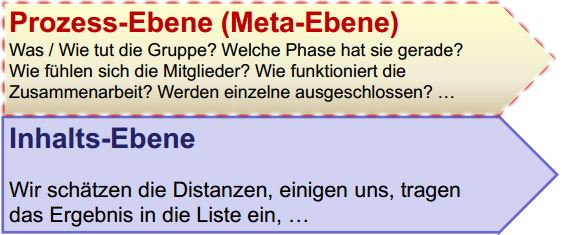
\includegraphics[width=0.5\linewidth]{fig/teamentwicklung-metaebene}
\caption{Teamentwicklung Ebenen}
\label{fig:teamentwicklung-metaebene}
\end{figure}

\paragraph{Vertrauen:} Vertrauen ist wie ein Baum. Wenn klein = sehr empfindlich. Wenn gross = stark und robust. Wächst langsam. Und man kann es nur kaputt machen.

\section{[MEP] Gruppenuhr}
Die Gruppenuhr durchläuft jedes Team. Kein Schritt ist überspringbar, doch schneller durchlaufbar. Ab und zu fallen Gruppen in frühere Phasen zurück. Der Prozess läuft immer wieder ab, auch verschachtelt. An jedem Meeting wieder neu. Sogar im Meetings teilweise pro Thema. Ziel ist es möglichst schnell in die performante Phase zu kommen, dies können wir gezielt und aktiv fördern. Hilfsmittel der Moderation und informellen Führung verwenden!

\begin{figure}[h!]
\centering
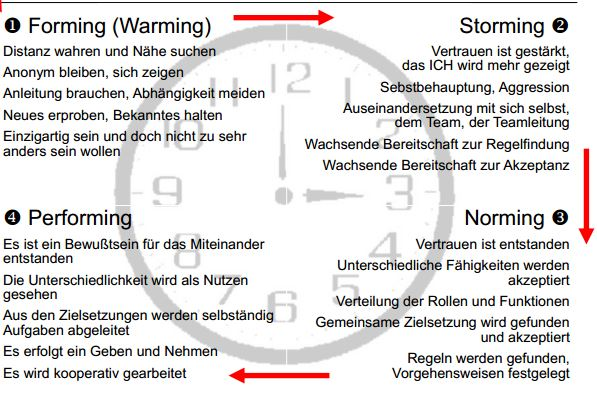
\includegraphics[width=0.7\linewidth]{fig/teamentwicklung-gruppenuhr}
\caption{Gruppenuhr}
\label{fig:teamentwicklung-gruppenuhr}
\end{figure}

\section{Grupenrollen}
In einem Team nehmen unterschiedliche Personen unterschiedliche Rolle ein, gewollt wie auch ungewollt. Nachfolgend einige Rollen: Gruppenführer, Beliebte, Tüchtige, Mitläufer, Opponent, Sündenbock, Aussenseiter. Bspw. gibt es immer einen Sündenbock. Wirft man diesen raus, gibt es einen Neuen.

\paragraph{Teamdesign} 
Untersuchungen zeigen, dass 8 bestimmte Aufgabentypen abgedeckt werden müssen, für ein erfolgreiches Team. Nach Charles Margerison \& Dick McCann sollte man die persönlichen Präferenzen ermitteln und sich so sein Team zusammenstellen. In der Praxis bekommt man meist jedoch ein Team, daher sollte man jedoch die am dafür geeignetsten Person für die Aufgabe ernennen. Jedes Team ist in acht Arbeitsfunktionen gegliedert um erfolgreich zu funktionieren (Beraten, Innovieren\dots). Diese werden den Mitgliedern zugeordnet und daraus ergeben sich die vier Arbeitspräferenzen (Rollen), die eine Person einnehmen möchte. Di Linking Skills in der Mitte sollte jedes Teammitglied beherrschen.

\begin{figure}[h!]
\centering
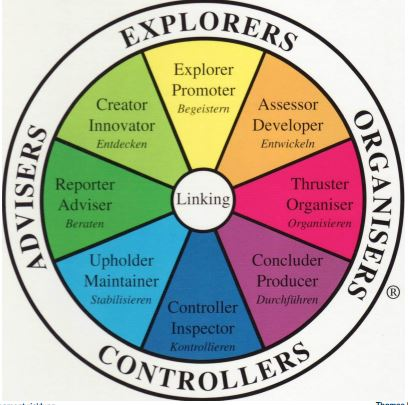
\includegraphics[width=0.5\linewidth]{fig/teamentwicklung-teamdesign-basismodell}
\caption{Teamdesign Basismodell}
\label{fig:teamentwicklung-teamdesign-basismodell}
\end{figure}

\section{Prognose}
In ein paar Jahren werden wir über das Postulat von Ernst Thomas reden: ''Kolosse sterben aus'', ''Chefs werden zu Netzwerkern'' und ''Globalisierung lässt sich nicht aufhalten''. Gestern: Schäferhund, treuer Angestellter. Heute: Husky, Teamplayer. Morgen: Katze, selbständig, vernetzt, kooperativ, kompetitiv, führbar und eigenbestimmt.